\section{Results}\label{sec:results}
\subsection{Ranking accuracy and protection quality}
Gradient scores associate more closely with positive isolated damage than significance alone on the sampled ResNet-8 and KWS bits (Table~\ref{tab:isolated}), but correlations remain moderate. ToyCar illustrates the importance of the objective: positive-gradient correlation is 0.637 for reconstruction-MSE damage, but 0.504 for AUC damage, close to absolute gradient's 0.501. Surrogate prediction quality is not a protection guarantee.

\begin{table}[t]
\caption{Spearman correlation with positive isolated damage on 320 shared stratified bits per model. ToyCar here uses the MSE surrogate, not task AUC. These are sample-design statistics.}\label{tab:isolated}
\centering\small
\begin{tabular}{lrrr}\toprule
Ranking & ResNet-8 & KWS & ToyCar MSE\\\midrule
Random & $-0.054$ & 0.012 & 0.059\\
MSB-first & 0.256 & 0.204 & 0.502\\
Numerical jump & 0.070 & 0.175 & 0.439\\
Global gradient & 0.364 & 0.258 & 0.498\\
Absolute gradient & 0.376 & 0.288 & 0.546\\
Positive gradient & 0.364 & 0.246 & 0.637\\\bottomrule
\end{tabular}
\Description{Moderate and task-dependent correlations between sampled exact isolated damage and six scores.}
\end{table}

Figures~\ref{fig:ber} and~\ref{fig:budget} show the task-level result. At BER 1\% and protection 12.5\%, ResNet-8 loss is 20.093 nats/image unprotected, 8.715 with MSB-first and 2.098 with absolute-gradient allocation. Pythia gives 22.019 nats/token unprotected, 12.706 with MSB-first and 7.883 with global gradient. Ranking choice therefore matters well beyond small networks.

ToyCar does not follow the same pattern: its risks at that condition are 0.261 unprotected, 0.337 with MSB-first and 0.308 with absolute gradient, against 0.131 clean. Its nonmonotonic curves reflect complete-file score ordering, not reconstruction error. DistilBERT sometimes has slightly lower loss than clean inference on its fixed cohort; this is not evidence that corruption generally improves the model.

\begin{figure}[tbp]
\centering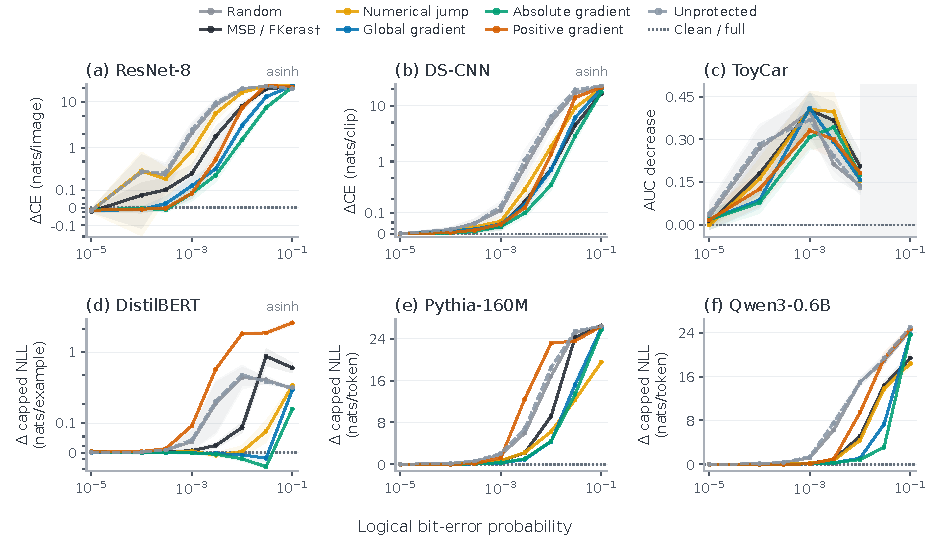
\includegraphics[width=\linewidth]{compact_reliability_ber_125}
\caption{Loss degradation versus BER at 12.5\% protection. Lower is better; bands are 95\% fault-field intervals and zero is clean/full protection. Panels use their own task units. Asinh denotes nonlinear vertical spacing with original-unit ticks. FKeras equals MSB at this complete tier on the three TFLite models only; it is unavailable for the transformers. Lines connect measured points.}\label{fig:ber}
\Description{Six compact panels comparing measured methods over BER, with unprotected and clean references.}
\end{figure}

\begin{figure}[tbp]
\centering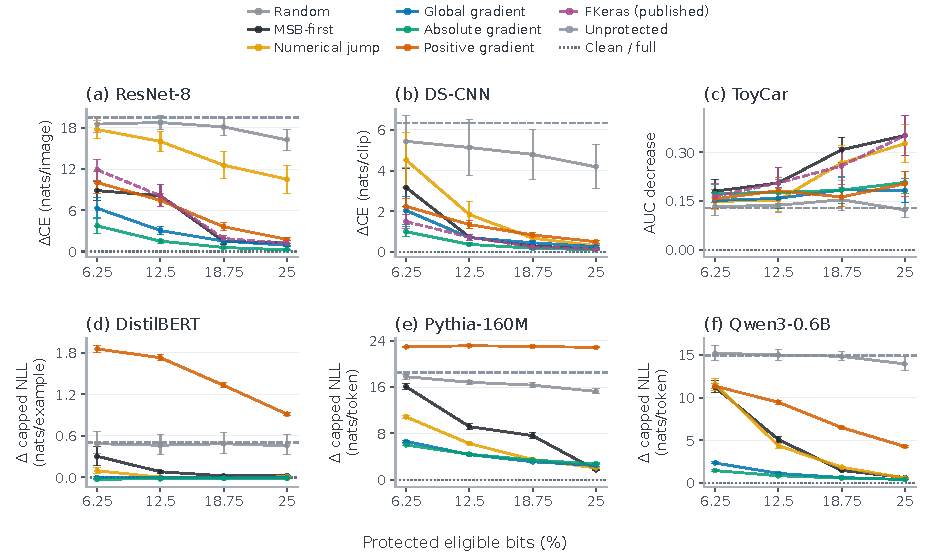
\includegraphics[width=\linewidth]{compact_reliability_budget_001}
\caption{Loss degradation versus protected fraction at BER 1\%. Error bars are 95\% field-level mean intervals. Horizontal references show unprotected and clean/full protection. Equal fractions refer to different eligible-bit populations, not equal hardware cost or absolute fault exposure.}\label{fig:budget}
\Description{Six compact budget panels including the partial-tier comparisons and task-specific uncertainty.}
\end{figure}

\subsection{Changes in method preference}
Paired contrasts, rather than overlapping marginal bands, establish the reversals in Table~\ref{tab:paired}. On Pythia, global gradient is better than MSB-first at 12.5\% coverage but worse at 25\%, for the same checkpoint, BER and cohort. At partial tiers, the Hessian-based allocation is better than MSB-first on KWS and worse on ResNet-8. At complete tiers their masks and outcomes coincide, so they are not independent alternatives.

\begin{table}[t]
\caption{Paired loss differences at explanatory conditions. Negative favors the first method. Units are nats per image, clip, or token. Original Holm families are retained; Qwen follow-up intervals are exploratory. Full grids accompany the paper.}\label{tab:paired}
\centering\small
\begin{tabularx}{\linewidth}{l r r X r}\toprule
Model; contrast & BER & Budget & Difference [95\% CI] & Holm $p$\\\midrule
KWS; FKeras $-$ MSB & .01 & 6.25\% & $-1.678$ [$-2.425,-.930$] & .0112\\
ResNet-8; FKeras $-$ MSB & .01 & 6.25\% & $+3.035$ [$1.835,4.234$] & .0112\\
Pythia; global $-$ MSB & .01 & 12.5\% & $-4.823$ [$-5.395,-4.343$] & .0160\\
Pythia; global $-$ MSB & .01 & 25\% & $+.771$ [$.553,1.025$] & .0160\\
Qwen; absolute $-$ MSB & .05 & 12.5\% & $-9.297$ [$-10.021,-8.567$] & ---\\
Qwen; absolute $-$ MSB & .075 & 12.5\% & $+1.637$ [$.605,2.661$] & ---\\\bottomrule
\end{tabularx}
\Description{Opposite paired method preferences across architectures, protection budgets and BERs.}
\end{table}

Qwen's follow-up reversal also appears in finite uncapped NLL: at BER 7.5\%, absolute gradient gives 23.149 versus 21.374 for MSB-first. However, 10.49\% and 7.07\% of finite token losses reach the 30-nat ceiling. The effect is not solely a capping artifact, but occurs under severe degradation. It does not identify a practical operating range or prove an interaction-driven transition.

\subsection{Monte Carlo-guided allocation}
Conditional selection changes the exact-isolated mask in 27 of 32 KWS pools. Its held-out mean difference is nevertheless only $-8.24\times10^{-5}$ nats/clip, with across-pool interval $[-0.00169,0.00153]$ and two-sided $p$-value 0.918 (Fig.~\ref{fig:decisions}). Eleven pools favor conditional selection, five tie and sixteen favor isolation. Thus, the changed decisions do not establish improved expected protection.

\begin{figure}[tbp]
\centering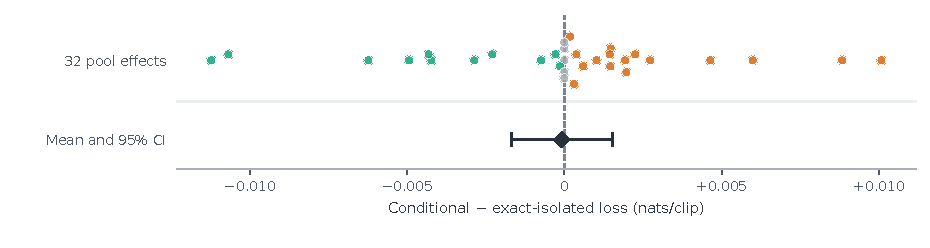
\includegraphics[width=.90\linewidth]{compact_kws_pools}
\caption{Held-out conditional-minus-exact-isolated loss across all 32 KWS pools at BER 5\%. Each dot is one pool; the diamond and bar show the mean and its 95\% pool-level interval. Negative favors conditional selection. Vertical offsets only separate overlapping dots. The mean does not resolve an advantage.}\label{fig:decisions}
\Description{All pool effects around zero, with an unresolved mean improvement and visible heterogeneity.}
\end{figure}

Both methods improve slightly over the original absolute-gradient mask: conditional selection by 0.00268 nats/clip, interval $[0.00058,0.00478]$, and isolation by 0.00248, interval $[0.00036,0.00459]$; both saved Holm-adjusted $p$ values are 0.0279. These separate paired estimates need not subtract exactly. The result supports a benefit from local reevaluation, not a unique benefit from conditioning. Exact interaction diagnostics in the appendix likewise show changed preferences without resolved conditional-over-isolated superiority.

\subsection{Computational cost}
Mean construction times for global gradient are 1.19/0.41/3.85 seconds on ResNet-8/KWS/ToyCar; rank-two Hessian scoring takes 5.58/1.43/11.42 seconds. Shared absolute/positive-gradient computation takes 16.99/7.47/208.43 seconds, excluding loading. Median wide-sweep evaluation times are 23.75, 11.56 and 32.55 seconds per DistilBERT, Pythia and Qwen request. Conditional selection requires $2^K$ evaluations per outside field. Its cost is therefore material even when the measured decision gain is small.
